\documentclass[11pt]{beamer}
\usepackage{amsmath}
\usepackage{amssymb}
\usepackage{amsthm}
\usepackage[utf8]{inputenc}
%\usepackage[margin=0.5in]{geometry}
\usepackage{graphicx}
\usepackage{algorithm}
\usepackage{algpseudocode}
\usepackage{xcolor,colortbl}
\usepackage{url}
\usepackage{caption}
%\usepackage{algorithmic}
\usepackage{algorithm}
\usepackage{comment}

\newcommand{\mc}[2]{\multicolumn{#1}{c}{#2}}
\definecolor{Gray}{gray}{0.85}

\newcolumntype{a}{>{\columncolor{Gray}}c}
\newcolumntype{b}{>{\columncolor{white}}c}


\newtheorem*{proposition}{Proposition}
\newtheorem*{proof_}{proof}

\DeclareMathOperator{\tw}{tw}
\DeclareMathOperator{\VC}{VC}
\DeclareMathOperator{\CLIQUE}{CLIQUE}
\DeclareMathOperator{\reach}{reach}

\title{final report for CS260: \\ \normalsize the vertex cover problem}
\author{Osayd Abdu (142461), Abdulelah Alneghaimish (159296), \\ Lukas Larisch (154273), Elaf Islam (142724)}
\date{}

\parindent 0pt


\begin{document}

\begin{frame}

\maketitle

\end{frame}

\begin{frame}
\frametitle{Motivation from theory}

\begin{theorem}[Courcelle, 1990]
Every graph property definable in monadic second-order logic can be decided in linear time on graphs of bounded treewidth.
\end{theorem}

\begin{itemize}
\item most problems from NP are definable in MSO
\item [] $\rightarrow$ max-CLIQUE
\item [] $\rightarrow$ min-VERTEX COVER
\item no experimental evaluation of this theorem yet
\end{itemize}

\end{frame}




\begin{frame}
\frametitle{Recap: Vertex Cover}

$C \subseteq V(G)$, such that $\{u, v\} \in E(G) \implies u \in C \lor v \in C$. \\

\begin{center}

{
\centering
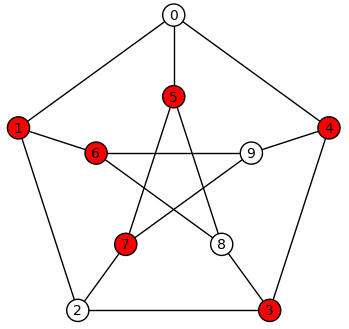
\includegraphics[scale=0.5]{example_cover}
}

\end{center}

\end{frame}


\begin{frame}
\frametitle{Recap: Clique}

$C \subseteq V(G)$, such that $u, v \in C \implies \{u, v\} \in E(G)$. \\


\begin{center}

{
\centering
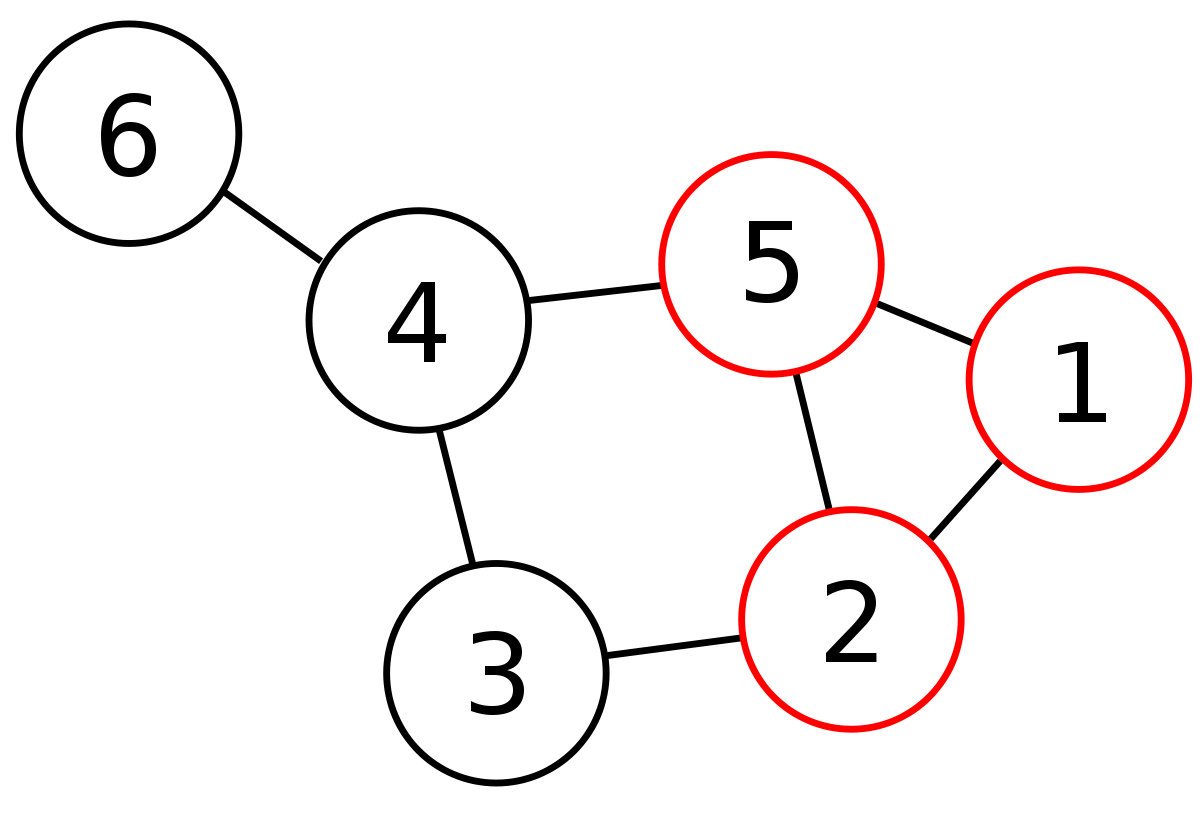
\includegraphics[scale=0.2]{example_clique}
}

\end{center}

\end{frame}


\begin{frame}
\frametitle{Recap: they are poly-time reducable}

$(G, k) \in \VC \iff (\bar G, |V(G)|-k) \in \CLIQUE$
\end{frame}


\begin{frame}
\frametitle{Recap: First algorithm}

\begin{itemize}
\item exponential time
\item Basically:
\begin{itemize}
\item For $v$, we investigate $v \in \CLIQUE$ and $v \not \in \CLIQUE$.
\item $v \in \CLIQUE$: Remove all vertices not connected to $v$ and recurse.
\item $v \not \in \CLIQUE$: Remove $v$ and recurse.
\vspace*{5mm}
\item [] $\rightarrow$ $\mathcal{O}(2^n \cdot \text{poly}(n))$
\end{itemize}
\end{itemize}

\end{frame}

\begin{frame}
\frametitle{Recap: Second algorithm}

\begin{itemize}
\item exponential time for unbounded treewidth
\item otherwise, $\mathcal{O}(2^{tw(G)+1} \cdot n^{O(1)}) = \mathcal{O}(n)$.

\item Compute a tree decomposition of minimum size for the input graph
\item Convert it to a nice tree decomposition (can be handled better in later steps)
\item Dynamic Programming on the nice tree decomposition (extension of approach on trees, see HW3 for Independent Set)
\end{itemize}

\end{frame}


\begin{frame}
\frametitle{Graphs}

\begin{itemize}
\item Control flow graphs
\item random partial $k$-trees 
\begin{itemize}
\item $k \in \{1, \dots, 15\}$
\item $n \in \{50,100,200,250,500\}$
\item $p \in \{.97, .95, .90, .80, .70\}$ 
\item 5 each
\end{itemize}
\item "named" graphs, e.g.
\begin{itemize}
\item Petersen 
\item world map graph (countries adjacent  $\rightarrow$ edge)
\end{itemize}
\end{itemize}
\end{frame}



\begin{frame}
\frametitle{Statistics: Control flow graphs}

\begin{center}
\footnotesize
\begin{table}[h!]
\centering
\begin{tabular}{|c|c|c|c|c|c|}
\hline
\#graphs & avg/med./max \#vert. & avg/med./max \#edges & avg/med./max $\tw$ \\
\hline \hline
142 & 37.47/23/544 & 39.45/24/609 & 1.85/2/4 \\
\hline
1082 & 36.49/19/1452 & 38.08/19/1591 & 1.71/2/7 \\
\hline
529 & 42.07/24/587 & 45.13/24/668 & 1.97/2/6 \\
\hline
\end{tabular}
\captionof{table}{Statistics for the considered CFGs.}
\label{stat_CFGs}
\end{table}
\end{center}

\end{frame}


\begin{frame}
\frametitle{Statistics: random partial $k$-trees (1)}

\begin{center}
\begin{table}[h!]
\centering
\begin{tabular}{|c|c|c|c|}
\hline
$n$ & avg/med./max \#edges & avg/med./max $\tw$ \\
\hline \hline
50 & 48.11/30/218 & 3.66/2/15 \\
\hline
100 & 102.11/61/441 & 4.46/3/15 \\
\hline
200 & 211.70/90/908 & 5.07/3/15 \\
\hline
250 & 264.48/153/1116 & 5.27/4/15 \\
\hline
500 & 537.28/310/2236 & 5.95/5/15 \\
\hline
\end{tabular}
\captionof{table}{Statistics for the considered partial $k$-trees grouped by $n$.}
\end{table}
\end{center}

\end{frame}


\begin{frame}
\frametitle{Statistics: random partial $k$-trees (2)}

\begin{center}
\small
\begin{table}[h!]
\centering
\begin{tabular}{|c|c|c|c|}
\hline
$k$ & avg/med./max \#edges & avg/med./max $\tw$ \\
\hline \hline
1 & 29.95/16/165 & 0.97/1/1 \\
\hline
2 & 60.70/30/329 & 1.40/1/2 \\
\hline
3 & 88.3/47/485 & 1.75/2/3 \\
\hline
4 & 118.58/62/626 & 2.30/2/4 \\
\hline
5 & 147.68/77/787 & 2.76/2/5 \\
\hline
6 & 178.70/94/936 & 3.43/3/6 \\
\hline
7 & 204.95/106/1082 & 4.09/4/7 \\
\hline
8 & 234.02/123/1189 & 4.79/5/8 \\
\hline
9 & 262.10/143/1370 & 5.31/6/9 \\
\hline
10 & 290.24/149/1492 & 6.06/7/10 \\
\hline
11 & 318.78/166/1658 & 6.70/8/11 \\
\hline
12 & 348.72/169/1836 & 7.46/8/12 \\
\hline
13 & 375.87/187/1976 & 8.04/9/13 \\
\hline
14 & 404.34/210/2050 & 8.82/10/14 \\
\hline
15 & 431.58/218/2236 & 9.45/11/15 \\
\hline
\end{tabular}
\captionof{table}{Statistics for the considered $k$-trees grouped by $k$.}
\end{table}
\end{center}

\end{frame}

\begin{frame}
\frametitle{Statistics: "named" graphs}

\begin{center}
\tiny
\begin{table}[h!]
\centering
\begin{tabular}{|c|c|c|c|c|c|}
\hline
package & \#graphs & avg/med./max \#vert. & avg/med./max \#edges & avg/med./max $\tw$ \\
\hline \hline
%all & 125 & 83.05/25/3282 & 166.63/60/6561 & 9.79/7/29 \\
$0 \leq \tw \leq 10$ & 85 & 73.74/19/3282 & 132.40/36/6561 & 5.40/5/10 \\
\hline
$11 \leq \tw \leq 20$ & 25 & 57.42/45/255 & 147.21/105/507 & 16.04/16/20 \\
\hline
$21 \leq \tw \leq 27$ & ? & 225.14/112/1023 & 481.71/210/2043 & 26.44/24/25 \\
\hline
\end{tabular}
\captionof{table}{Statistics for the named graphs.}
\end{table}
\end{center}

\begin{center}
\begin{figure}[h!]
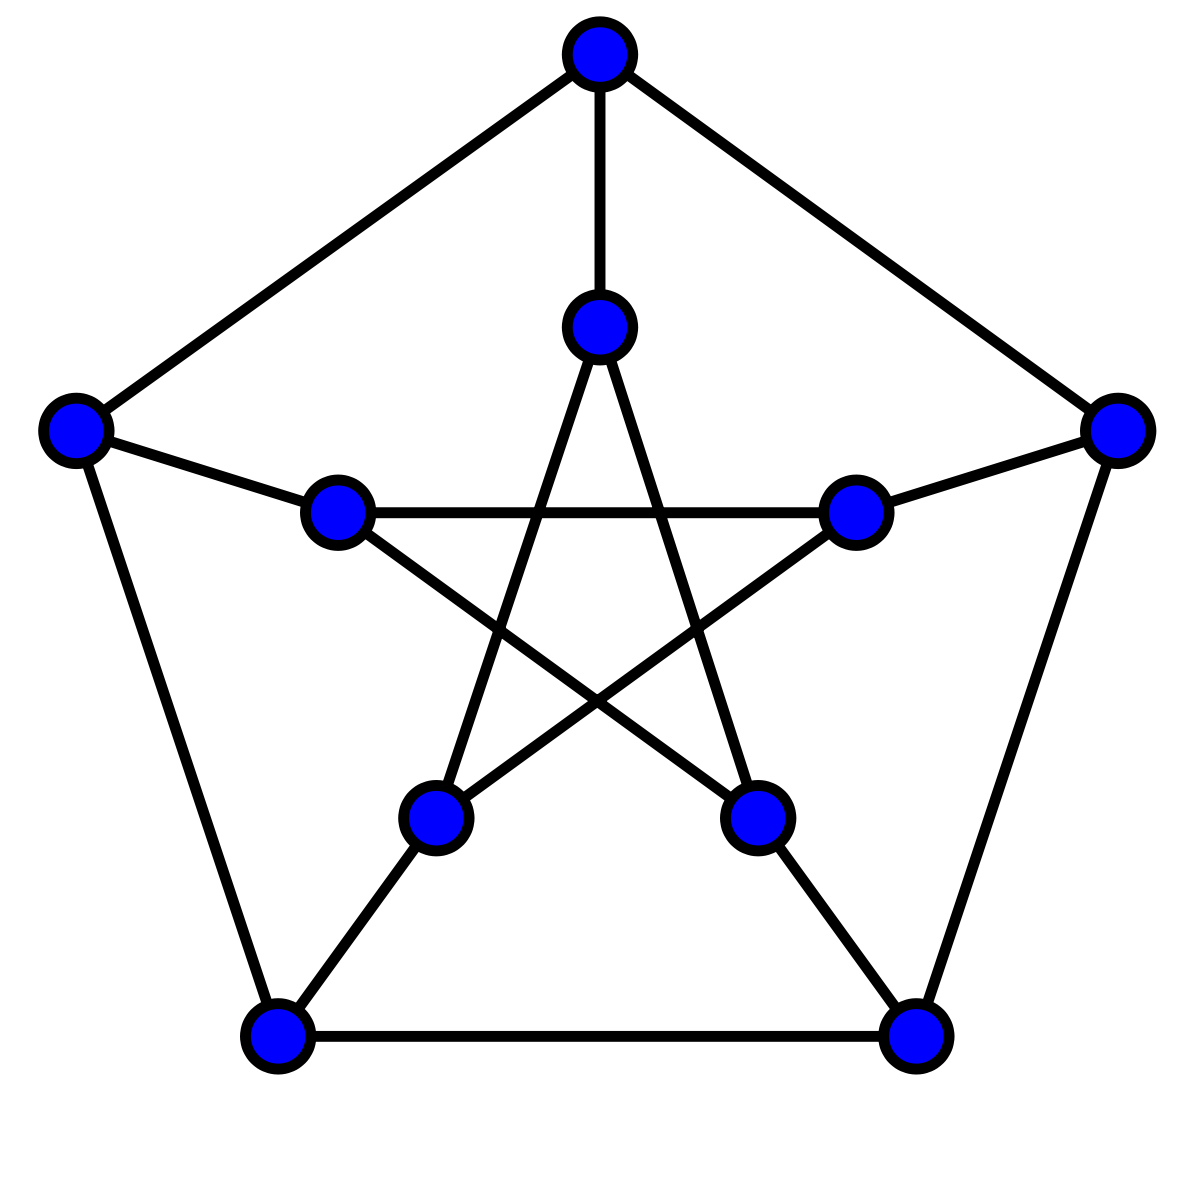
\includegraphics[scale=0.06]{Petersen}
\hspace*{3mm}
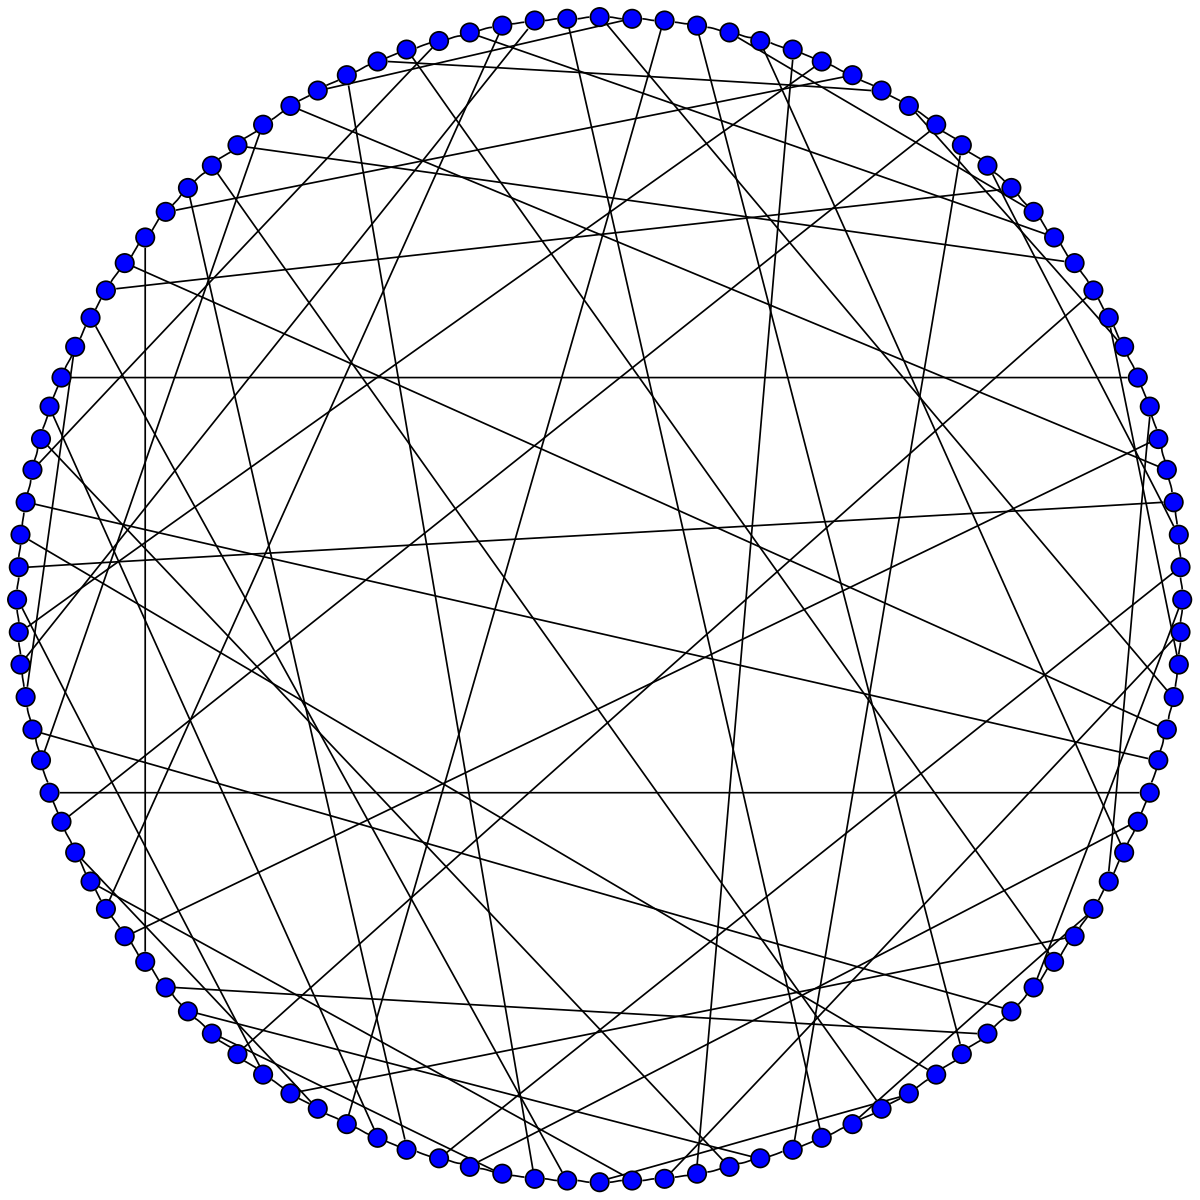
\includegraphics[scale=0.06]{Balaban}
\hspace*{3mm}
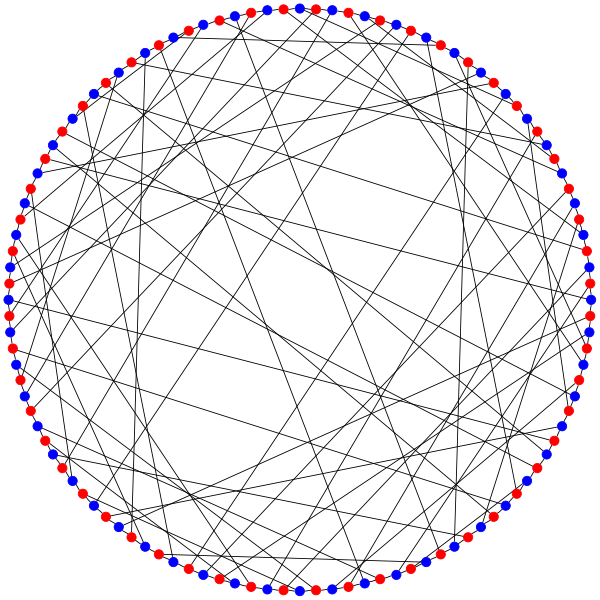
\includegraphics[scale=0.12]{Ljubljana}
\hspace*{3mm}
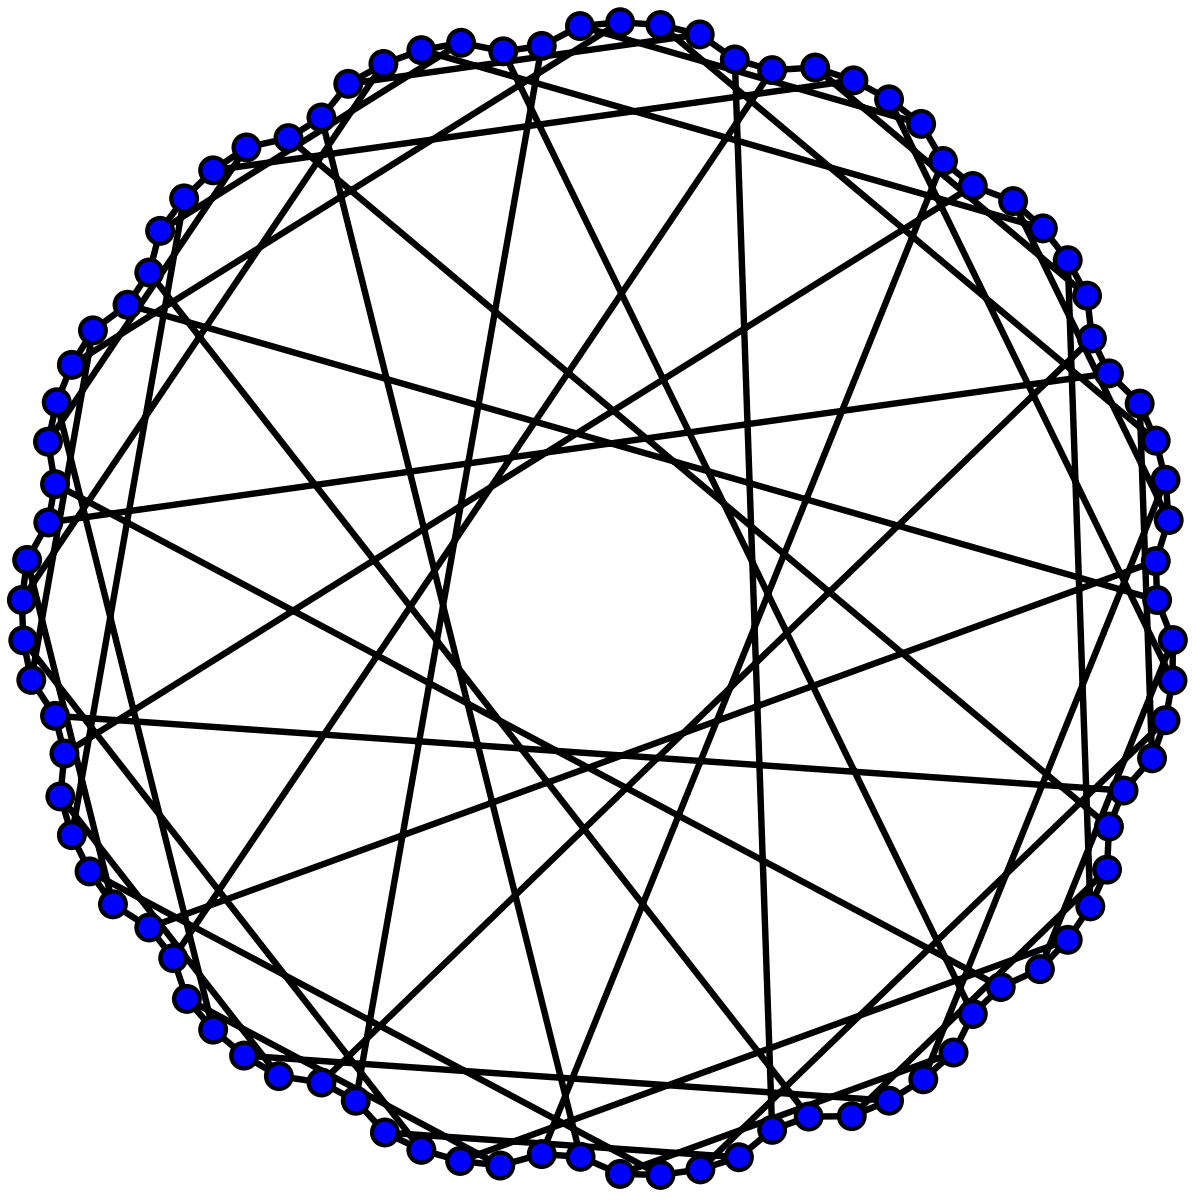
\includegraphics[scale=0.06]{Foster}
\caption{The Petersen, Balaban 11-cage, Ljubljana and Foster graphs.}
\end{figure}
\end{center}

Treewidths: treewidth 4, treewidth 25, treewidth 25, treewidth 22.

Last three are hardest for experiments.

\end{frame}


\begin{frame}
\frametitle{Experiments}

\begin{itemize}
\item C++ \& python
\item boost graphs \& networkx
\item TdLib for the provision of tree decompositions in algo 2 (won PACE 2017)
\item no graphs of treewidth $>$ 30
\end{itemize}
\end{frame}
\begin{frame}
\frametitle{Testing for Correctness}
We tested the correctness of our algorithms on these different types of graphs:
\begin{itemize}
	\item Path graph (e.g. $P_6$)
	\item Complete graph (e.g. $K_5$)
	\item Petersen graph and double Petersen graph
	\item Wagner graph
	\item Pappus graph
	\item Grid graph (e.g. 5 by 5 grid)
	\item Corner cases:
	\begin{itemize}
		\item Empty graph
		\item One node graph
		\item Edgeless graph
	\end{itemize}
\end{itemize}
\end{frame}
\begin{frame}
\frametitle{Results (algo 1): Control flow graphs}

\begin{center}
\footnotesize
\begin{table}[h!]
\centering
\begin{tabular}{|c|c|c|}
\hline
\#graphs & avg/med./max time[s] \\
\hline \hline
125 & 8.1831/0.0024/444.4748 \\
\hline
943 & 16.3669/0.0014/1463.5199 \\
\hline
436 & 2.7926/0.0027/846.7689 \\
\hline
\end{tabular}
\captionof{table}{Results for the considered CFGs.}
\end{table}
\end{center}

\begin{itemize}
\item Difference between median, mean and max is huge (e.g. avg $\approx 11690\times$median in line 2)
\end{itemize}

\end{frame}



\begin{frame}
\frametitle{Results (algo 1): random partial $k$-trees (1)}

\begin{center}
\footnotesize
\begin{table}[h!]
\centering
\begin{tabular}{|c|c|c|c|}
\hline
$n$ & avg/med./max \#V. & avg/med./max \#E & avg/med./max time[s] \\
\hline \hline
8 & 6.0733/7/8 & 5.1233/6/8 & 0.0004/0.0003/0.0017  \\
\hline
13 & 10.8904/11/13 & 10.2591/10/15 & 0.0007/0.0007/0.0024 \\
\hline
21 & 17.3654/17/21 & 17.2724/17/24 & 0.0020/0.0018/0.0090 \\
\hline
34 & 26.9601/27/34 & 27.9635/28/38 & 0.0115/0.0076/0.0720  \\
\hline
34+ & 48.1595/46/72 & 51.1329/49/82 & 58.7046/0.1344/1463.5199  \\
\hline
\end{tabular}
\captionof{table}{Results for CFGs grouped by $n$.}
\end{table}
\end{center}

Running time is exponential. Estimated time to run the remaining graphs is more than 150 hours.

\end{frame}


\begin{frame}
\frametitle{Graph of group 5 in log scale}
\begin{figure}
  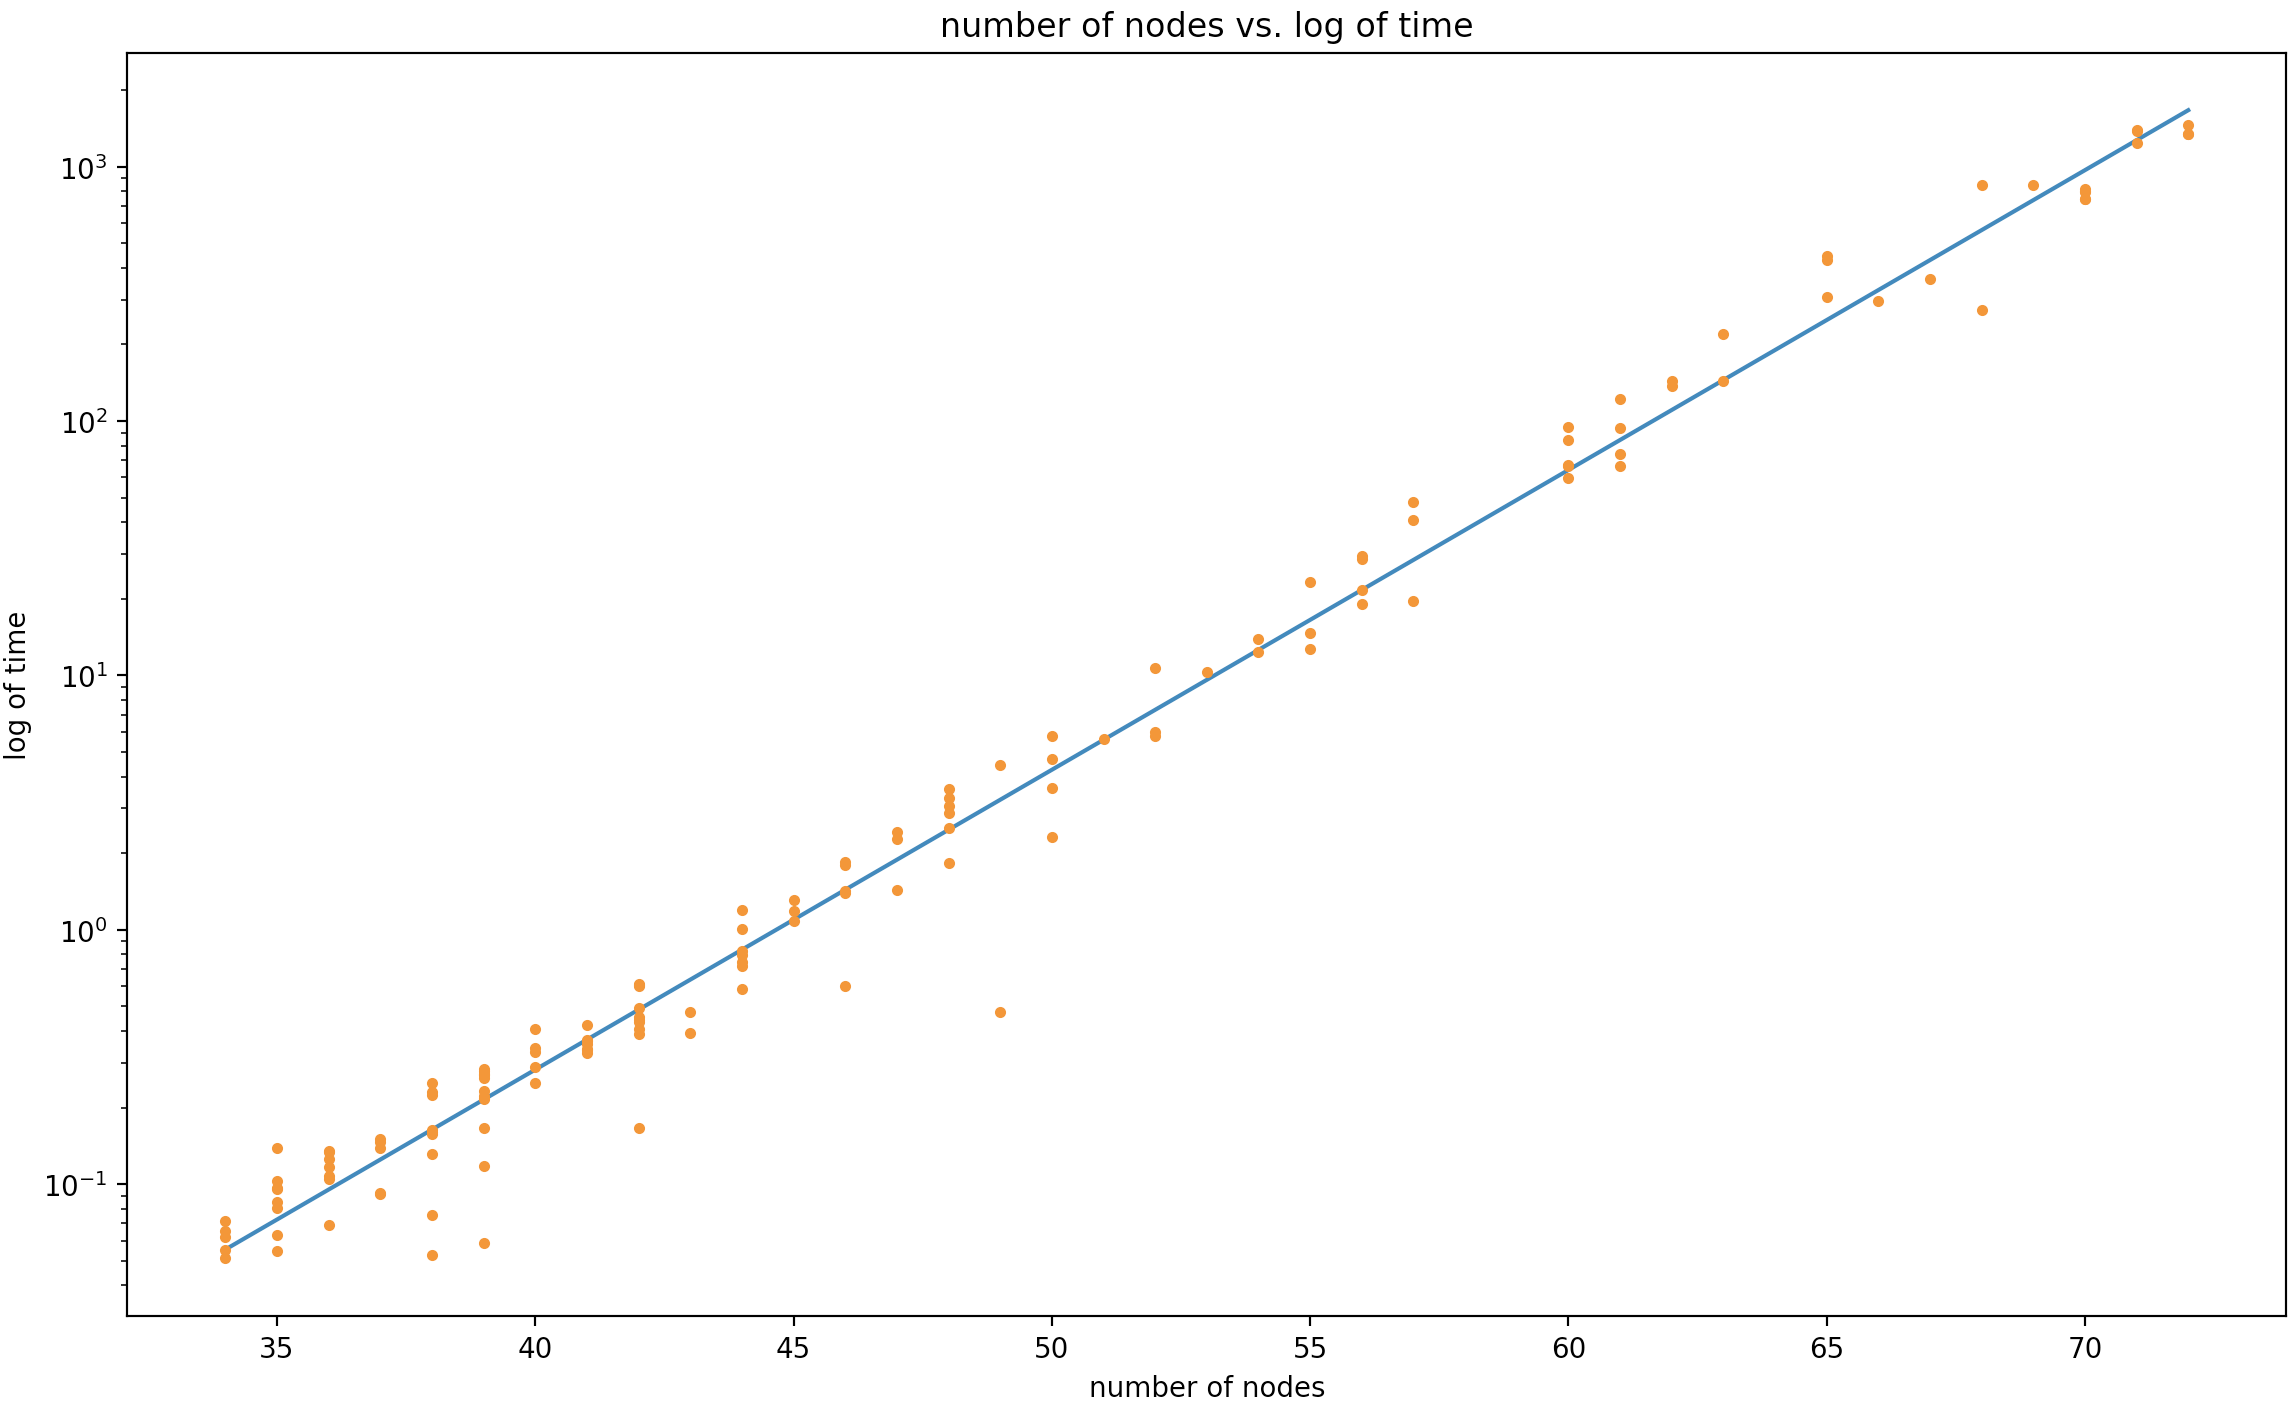
\includegraphics[width=\linewidth]{log.png}
  \caption{Nodes vs. Time (log scale)}
  \label{fig:log}
\end{figure}

\end{frame}
\begin{frame}
\frametitle{Graph of group 5 }
\begin{figure}
  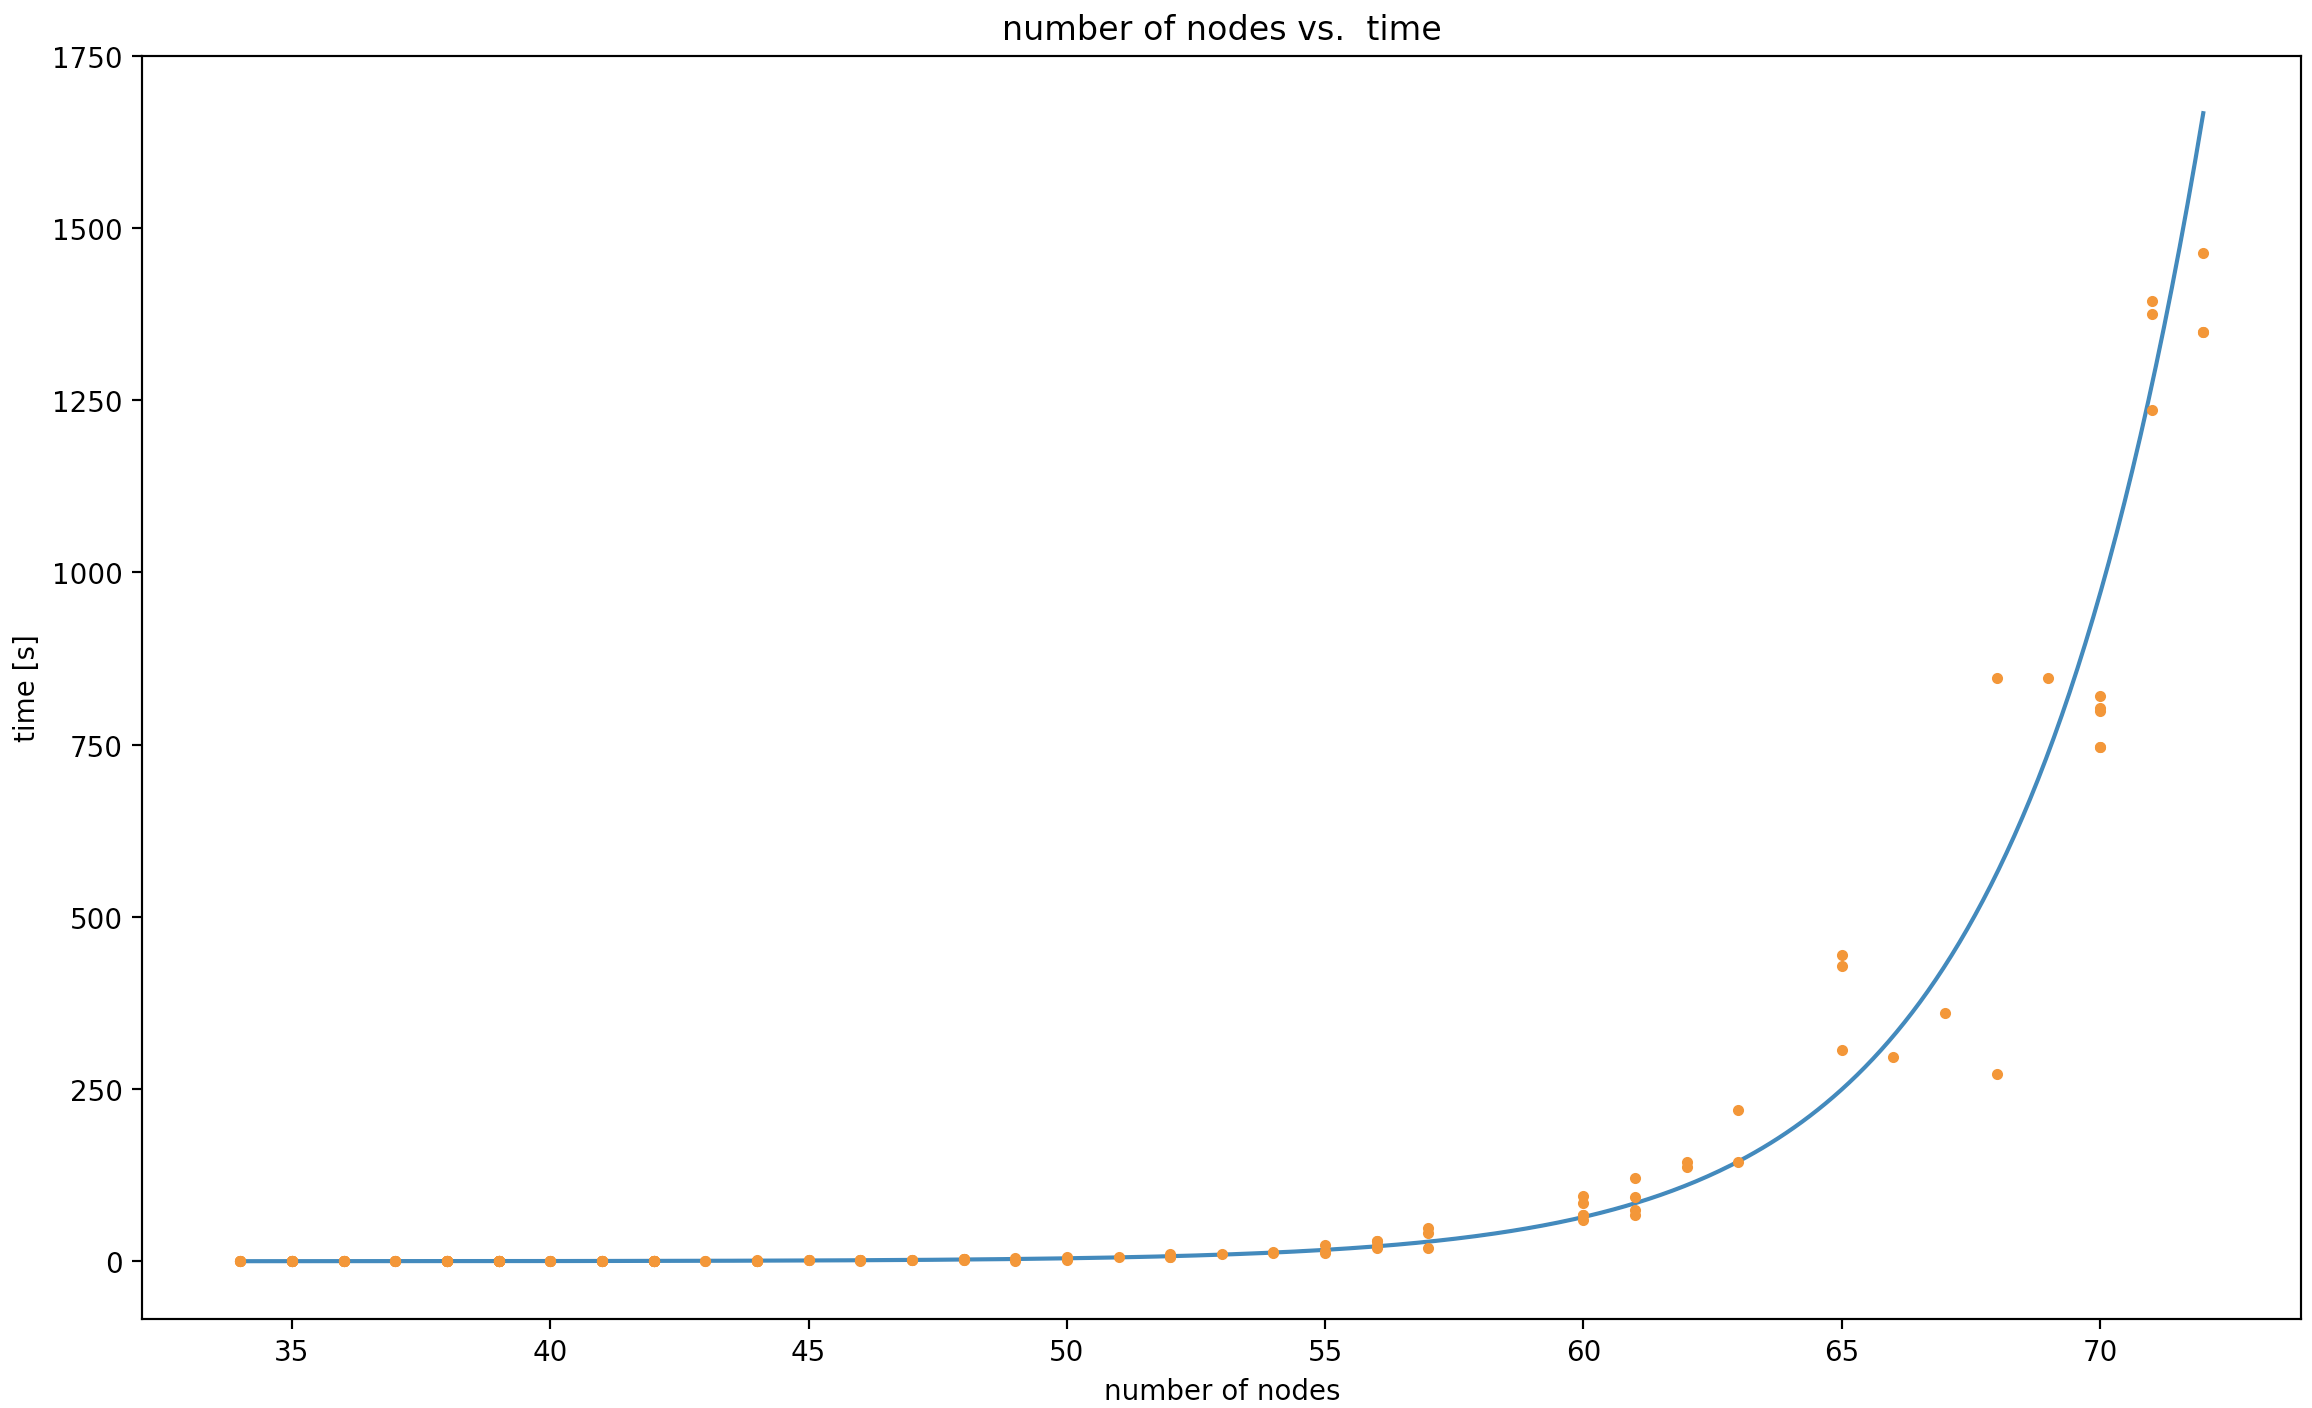
\includegraphics[width=\linewidth]{exp.png}
  \caption{Nodes vs. Time[s]}
  \label{fig:log}
\end{figure}
\end{frame}

\begin{frame}
\frametitle{Results (algo 2): Control flow graphs}

\begin{center}
\footnotesize
\begin{table}[h!]
\centering
\begin{tabular}{|c|c|c|c|c|c|}
\hline
\#graphs & avg/med./max $\tw$. & avg/med./max $\VC$ & avg/med./max time[s] \\
\hline \hline
142 & 1.85/2/4 & 18.56/11/269 & 0.0008/0.0003/0.0307 \\
\hline
1082 & 1.71/2/7 & 18.07/9/728 & 0.0007/0.0002/0.1559 \\
\hline
529 & 1.97/2/6 & 20.76/12/295 & 0.0008/0.0003/0.0339 \\
\hline
\end{tabular}
\captionof{table}{Results for the considered CFGs.}
\end{table}
\end{center}

\begin{itemize}
\item all graphs in less than 1 second
\item low treewidth (bounded by 7 + \#gotos)
\end{itemize}

\end{frame}



\begin{frame}
\frametitle{Results (algo 2): random partial $k$-trees (1)}

\begin{center}
\footnotesize
\begin{table}[h!]
\centering
\begin{tabular}{|c|c|c|c|c|}
\hline
$n$ & avg/med./max $\tw$. & avg/med./max $\VC$ & avg/med./max time[s] \\
\hline \hline
50 & 3.66/2/15 & 12.23/12/27 & 0.1347/0.0012/2.6110 \\
\hline
100 & 4.46/3/15 & 20.35/20/44 & 0.2666/0.0019/11.5305 \\
\hline
200 & 5.07/3/15 & 34.99/33/69 & 0.7391/0.0033/23.1289 \\
\hline
250 & 5.31/4/15 & 42.45/39/88 & 0.9472/0.0103/24.0645 \\
\hline
500 & 5.95/5/15 & 78.49/72/157 & 2.2913/0.0298/43.4646 \\
\hline
\end{tabular}
\captionof{table}{Results for the considered partial $k$-trees grouped by $n$.}
\end{table}
\end{center}

Running time linear in $n$.

\end{frame}


\begin{frame}
\frametitle{Results (algo 2): random partial $k$-trees (2)}

\begin{center}
\footnotesize
\begin{table}[h!]
\centering
\begin{tabular}{|c|c|c|c|c|}
\hline
$k$ & avg/med./max $\tw$. & avg/med./max $\VC$ & avg/med./max time[s] \\
\hline \hline
1 & 0.97/1/1 & 18.33/11/86 & 0.0042/0.0029/0.0130 \\
\hline
2 & 1.4/1/2 & 26.07/19/117 & 0.0036/0.0022/0.0127 \\
\hline
3 & 1.75/2/3 & 29.4/19/118 & 0.0043/0.0028/0.0195 \\
\hline
4 & 2.3/2/4 & 33.05/23/129 & 0.0064/0.0031/0.0309 \\
\hline
5 & 2.76/2/5 & 34.94/24/134 & 0.0096/0.0038/0.0525 \\
\hline
6 & 3.43/3/6 & 37.14/27/143 & 0.0171/0.0045/0.1015 \\
\hline
7 & 4.09/4/7 & 38.28/29/146 & 0.0308/0.0081/0.1774 \\
\hline
8 & 4.79/5/8 & 39.62/30/144 & 0.0542/0.0116/0.4428 \\
\hline
9 & 5.31/6/9 & 41.00/32/144 & 0.1058/0.0150/0.9290 \\
\hline
10 & 6.06/7/10 & 42.64/32/148 & 0.1780/0.0280/1.3136 \\
\hline
11 & 6.70/8/11 & 42.45/39/88 & 0.3626/0.0272/2.8060 \\
\hline
12 & 7.46/8/12 & 44.33/35/147 & 0.7838/0.03882/8.2476 \\
\hline
13 & 8.04/9/13 & 44.92/35/154 & 1.5113/0.0586/12.1212 \\
\hline
14 & 8.82/10/14 & 45.42/36/146 & 3.7556/0.1338/42.6301 \\
\hline
15 & 9.45/11/15 & 47.46/38/157 & 6.2944/0.2169/44.1330 \\
\hline
\end{tabular}
\captionof{table}{Results for the considered partial $k$-trees.}
\end{table}
\end{center}

\end{frame}


\begin{frame}
\frametitle{Results (algo 2): "named" graphs}

\begin{center}
\tiny
\begin{table}[h!]
\centering
\begin{tabular}{|c|c|c|c|c|}
\hline
package & avg/med./max $\tw$. & avg/med./max $\VC$ & avg/med./max time[s] \\
\hline \hline
$0 \leq \tw \leq 10$ & 5.40/5/10 & 30.36/11/1095 & 0.0111/0.0017/0.5071 \\
\hline
$11 \leq \tw \leq 20$ & 16.04/16/20 & 36.08/24/170 & 31.3456/1.7467/447.1208 \\
\hline
$21 \leq \tw \leq 25$ & 26.44/24/25 & 140.29/56/682 & 2469.1672/2219.0984/7198.5197 \\
\hline
\end{tabular}
\captionof{table}{Results for the considered partial $k$-trees.}
\label{results_named}
\end{table}
\end{center}

\begin{itemize}
\item many "hard" graphs
\item For hardest graph: 
\begin{itemize}
\item $1000 \cdot 2^{26}$ stored entries
\item before applying "tricks": 4TB RAM necessary
\item after applying "tricks": just 40GB RAM necessary
\item  $>$ 70 billion computations
\item running time: 2 hours
\end{itemize}
\item 3 graphs having $26 \leq \tw \leq 30$ could be solved in less than one day.
\end{itemize}

\end{frame}


\begin{frame}
\frametitle{Conclusions}

\begin{itemize}
\item TD-based algos may be of practical use for solving NP-complete problems
\item exp-time algos perform poorly on most graphs, they do not use the structure of graphs
\vspace*{0.3cm}
\item [] $\rightarrow$ When your problem is to hard in terms of complexity, consider using structural properties like treewidth.
\vspace*{0.3cm}
\item [] Many graphs from real-world problems are structural simple
\begin{itemize}
\item $\VC$ for train infrastructure
\item [] $\rightarrow$ min-$\VC$ is min. number of stations that must run to use all tracks
\item but: train network usually have a large grid minor $\rightarrow$ large treewidth
\item use another structural property: train networks are almost planar
\item [] $\rightarrow$ there are efficient algorithms for many problems on planar graphs
\end{itemize} 
\end{itemize}

\end{frame}



\end{document}